\subsection*{Abstract}
\paragraph{}This document outlines a method for inferring correlates of protection against infection using serological data. Many studies infer i) prevalence from serological data using seropositivity thresholds (titre above a pre-defined value) or ii) incidence rates using seroconversion thresholds (change in titre between two-time points above a pre-defined value). These threshold values are determined from empirical data from previous studies and are often used as a fixed heuristic for identifying infection across all individuals. However, seropositivity and seroconversion rates for many pathogens vary according to host factors (e.g. age, infection history, sex) and time since infection, meaning using these fixed thresholds may lead to incorrectly estimated seroprevalence and seroincidence rates. Antibody kinetic modelling can account for individual-level variability arising from host factors and time since infection. Here, a two-phase antibody kinetic function is defined: one function for the infected individuals and a function for the non-infected individuals. Using this, it is possible to probabilistically determine the likelihood of infection based on the change in titre between two bleeds. Using these inferences, we can determine a functional form for the correlate of protection: the probability of infection for a given titre value at exposure. However, as this correlate influences the probability of infection given a titre, it will also influence the probability that an individual is in the infection or non-infection state, influencing the antibody kinetics of an individual. In addition, to determine a correlate of protection, we must identify individuals who were exposed (have the potential to be infected if they had no existing immunity) but not infected, which can be challenging to determine with surveillance data. Here, we derive a reversible-jump MCMC (RJ-MCMC) algorithm, which can use serological data to infer i) the two-phase antibody kinetics, ii) the correlate of protection, and iii) the probability of infection and exposure within one statistical framework (\textbf{Figure~\ref{fig:sch_A}}). We show that this algorithm can consistently recover the correlate of protection against infection on multiple simulated serological datasets.  

\begin{figure}[H]
    \centering
    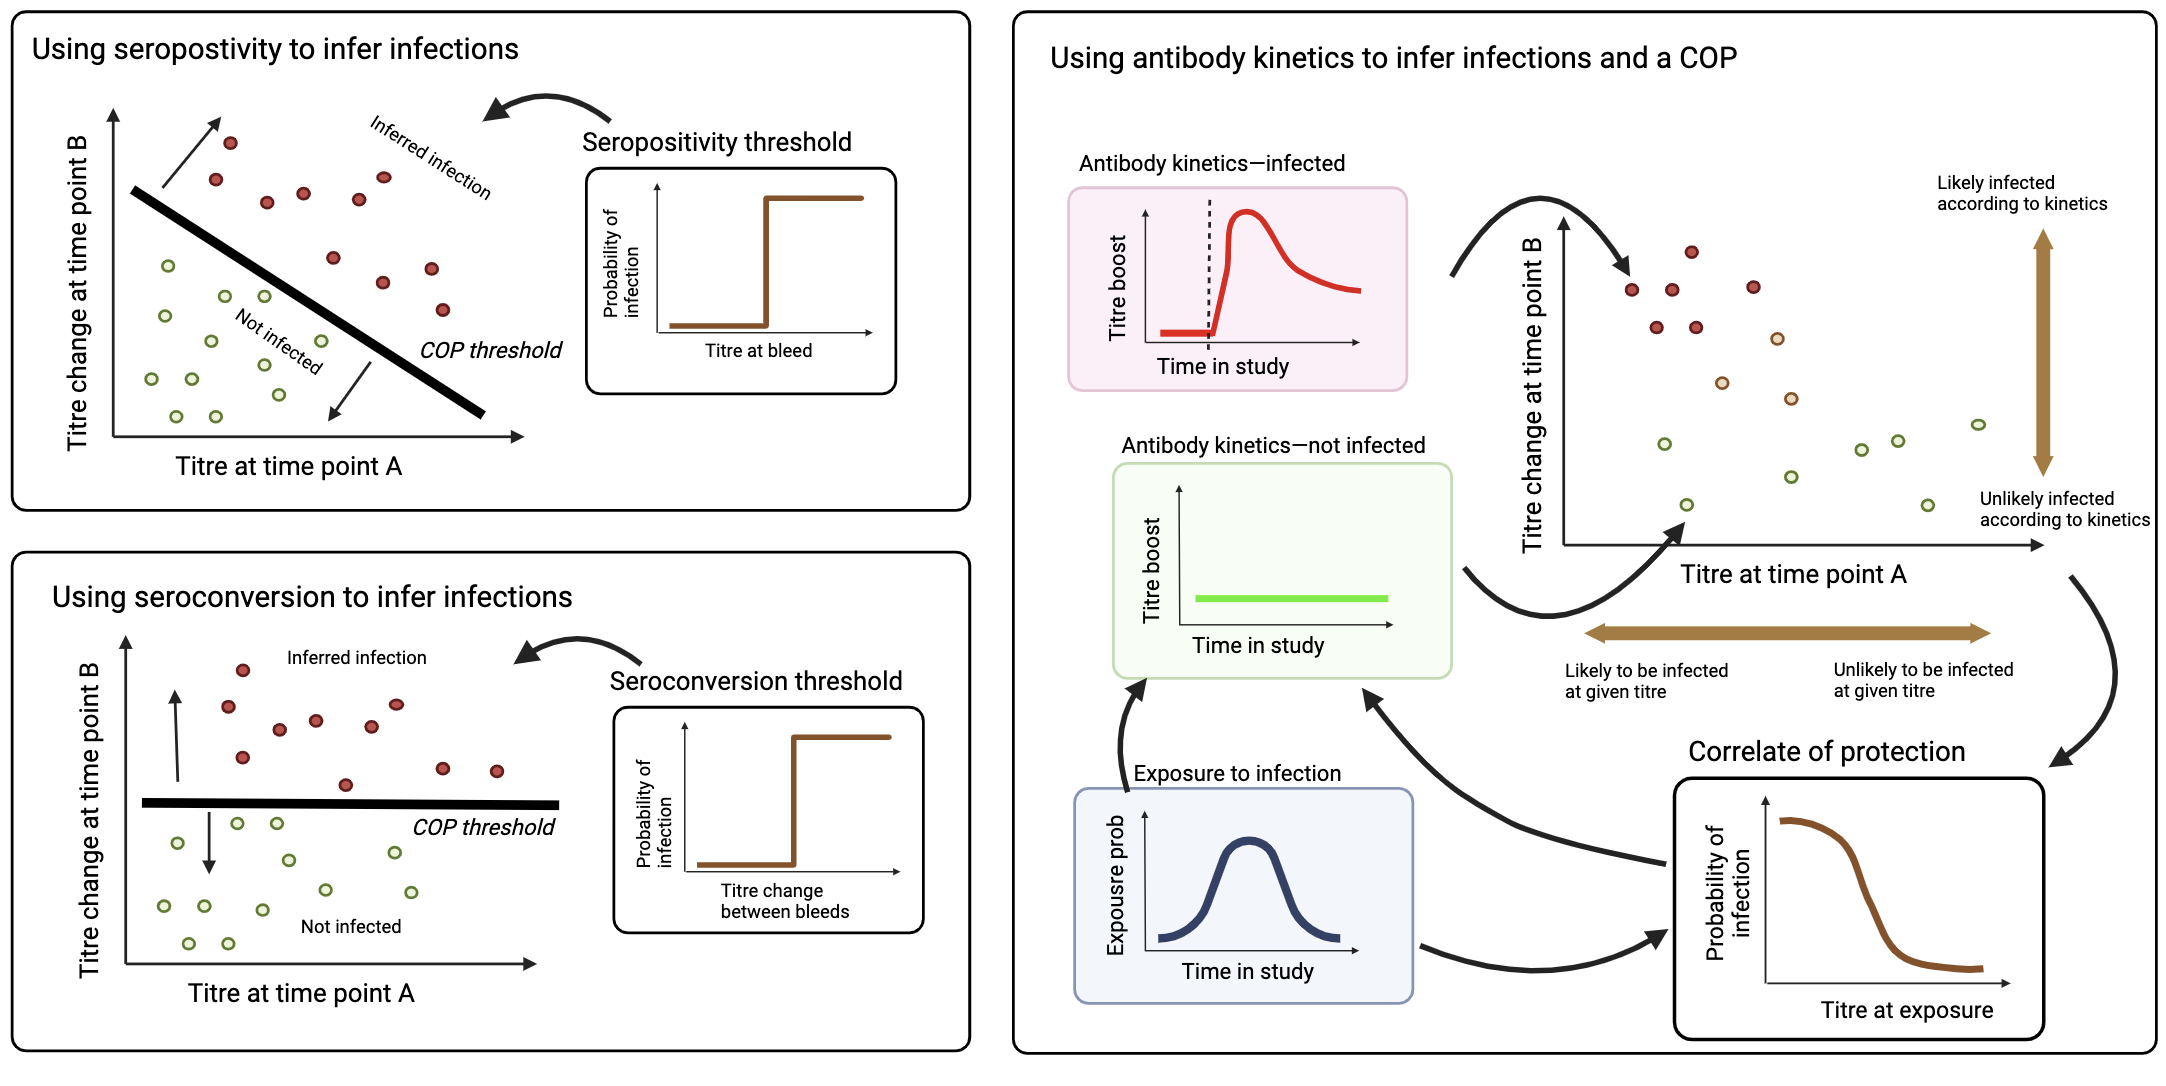
\includegraphics[width=1\textwidth]{sections/s1_intro/figs/sch_A.png}  \caption{Schematic showing how to use seropositivity, seroconversion, and antibody kinetics can be used to infer infections and in the case of antibody kinetics, also infer correlates of protection    \label{fig:sch_A}}
\end{figure}


\section{Overview of serological modelling}
\subsection{Introduction}

\paragraph{}Serological samples can be analysed to detect the presence of biomarkers made in response to an infection long after the infection has cleared.\cite{Cutts2016-za} Therefore, analysing serological samples allows researchers and healthcare professionals to deduce crucial information about the epidemiology of a pathogen at the individual and population level, which active virological surveillance systems may otherwise miss.

\paragraph{}On the individual level, after measuring antibodies to a specific pathogen, infection is usually inferred using either i) an antibody threshold level (seropositive) or ii) a threshold fold-rise between a pair of samples (seroconverted).\cite{Haselbeck2022-ob} Often, researchers are interested in understanding how seropositivity and seroconversion rates change according to controlled host factors, such as age, geography, living conditions, sexual behaviour, etc.\cite{Dhar-Chowdhury2017-yi, Wansom2021-jh, Crawford2006-wt} On the population level, serological samples which are representative of a population (e.g. cross-sectional samples) can be used to estimate the prevalence of infectious diseases (seroprevalence) and determine how seroprevalence changes over time according to host factors.\cite{Chan2021-me,Van_den_Berg2023-pl,Colton2021-bt} Estimates of seropositivity, seroconversion, and seroprevalence can help the understanding of the immune system's ability to combat various pathogens, aid in developing new targeted intervention programmes and provide insights into the transmission dynamics of infectious diseases. The methods used to analyse serological samples to inform epidemiology and public health policy of infectious diseases have been termed 'serodynamics' and have recently been reviewed.\cite{Hay2023-ty}

\paragraph{}Serological samples play an increasingly important role in public health efforts to combat and control infectious diseases.\cite{Haselbeck2022-ob,Metcalf2016-tr} However, inferring infection through seropositivity or seroconversion requires deriving an absolute or relative threshold value, and these are often determined by rule-of-thumb heuristics (e.g. for influenza: 4-fold-rise for conversion, titre of 1:40 HAI for seropositivity).\cite{Xu2021-pz} However, antibody responses vary greatly between individuals for many pathogens. Therefore, relying on these heuristics to determine infections in serology studies can lead to incorrect infection status being inferred, leading to biased estimates of prevalence.\cite{Chan2021-me,Cauchemez2012-ui} Consequently, a better understanding of the kinetics of antibody trajectories post-vaccination and infection can help assess the accuracy of existing heuristics and better inform infection status.

\subsection{Antibody kinetics}

\paragraph{}Modeling antibody kinetics involves using mathematical and statistical techniques to simulate the trajectories of antibodies in response to an infection or vaccination.\cite{Hay2023-ty} Typically, this involves using mathematical equations and statistical methods to describe the time-dependent changes in antibody levels within an individual or a population. This process is essential for understanding how antibody levels evolve and, therefore, potentially protect against infectious diseases. Various functional forms have been used to model the individual-level kinetics of antibody trajectories,\cite{Garcia-Fogeda2023-yc, Ranjeva2019-go, Hay2019-xu, Srivastava2023-of,Zhao2018-op,Teunis2016-wh} typically it follows a three-stage process:

\begin{itemize}
\item \textit{Initial} Response: The trajectories start by capturing the initial antibody response to a pathogen or vaccine. A rapid increase in antibody levels characterises this phase as the immune system recognises and mounts a defence against the antigen. The speed and relative contributions of memory versus de novo responses depend on whether the exposure is primary or secondary.

\item \textit{Peak Antibody Level}: The trajectories then rise to a peak antibody level, the highest antibody concentration reached during the immune response. This peak can vary depending on factors like the strength of the immune response and the route of and composition of antigen(s) in the exposure.

\item \textit{Decay Phase}: After the peak, there is a decline in antibody levels and the plasmablasts which secrete them. Therefore, antibodies have a finite half-life in the bloodstream, and their concentration gradually decreases as the pathogen is cleared or the vaccine antigen wanes. Over time, antibodies are continuously secreted from newly established long-lived plasma cells. Therefore, decay phase trajectories often converge to a set-point titre or a slow long-term waning rate.\cite{Srivastava2023-of, Amanna2010-zh, Andraud2012-ci}
\end{itemize}


\paragraph{}Modeling antibody kinetics provides several important benefits. First, by understanding the rate of antibody decline, models can estimate how long an individual's immunity is likely to last after infection or vaccination. Kinetics also help optimise vaccination strategies and identify the optimal timing and frequency of booster vaccinations to maintain protective antibody levels within a population. This is especially important for vaccine-preventable diseases with varying immunity levels, such as influenza and COVID-19.

\subsection{Correlates of protection}
\paragraph{} A correlate of protection (COP), defined here, is an immune function or biomarker that predicts protection against infection by a pathogen of interest. Studies such as vaccine trials often estimate thresholds of protection from disease (i.e. >50\% probability) for immune biomarkers, and these thresholds exist for influenza, Hepatitis A and B, Measles, Polio, Rabies, Yellow fever and more.\cite{Plotkin2022-pg} Vaccine trials which estimate thresholds of protection do not estimate the titre value at the time of exposure and, indeed, cannot estimate which individuals were even exposed to the pathogen throughout the trial. Therefore, though estimating thresholds of protection from disease is pivotal in designing and optimising vaccines to induce the required immune response effectively, they cannot be used to estimate the COP as defined. \cite{Immunology_undated-fs}

\paragraph{}Determining the immunological profiles of individuals exposed to an infection but managed to abort it is crucial for determining a universal correlate of protection. Usually, these individuals are identified through challenge studies, where their immune profiles are measured and challenged with live viruses.\cite{Deming2020-rz} As all individuals in the study have been exposed to the virus, it is then possible to determine which biomarkers correlate with protection from infection and disease. However, it's unclear how applicable these estimates are for real-world exposures, as we don’t know the typical infecting dose of a pathogen. The studies are also performed on fit and healthy individuals, which are not representative of the population vulnerable to severe infection by infectious disease. Finally, these studies focus on finding threshold values corresponding to 50\% protection from infection and diseases and it is unclear what the protection dynamics are for individuals outside this range. Further, these studies are also expensive, difficult to run, and are only possible for pathogens with mild pathogenesis.\cite{Sekhar2020-ux} 

%  https://www.nature.com/articles/s41591-022-01721-6
\paragraph{}Using serological samples to establish a correlate of protection would solve the aforementioned problems with challenge studies as they are cheaper to conduct, more inclusive, and can be used for any circulating virus in a population. A natural biomarker for a correlate of protection from infection is the amount of neutralising antibodies in the serum, which measures a serum's ability to prevent viral particles from infecting vulnerable cells. Therefore, those with high levels of neutralising antibodies could abort an infection by neutralising viral particles in-host even if exposed to a virus. However, determining correlates of protection through serological studies and measuring neutralising capacity is challenging because those exposed but experiencing an abortive infection generally leave no measurable antibody imprint and cannot be identified through serological testing.\cite{Swadling2023-ud}  Therefore, serological studies can be augmented with either immunological profiling to determine other immunological biomarkers that indicate 'abortive' infection\cite{Swadling2022-yv} or include intensive contact tracing with the serological studies to determine exposure rates between individuals.\cite{Cohen2022-sy} Augmented serological studies increase their complexity and cost and, therefore, are not feasible in many settings. Using existing study designs, there is a need for new statistical and mathematical methods for inferring latent epidemiological parameters, such as past infections and correlates of protection.
  

\subsection{Overview of modelling framework}
\paragraph{}Previous studies have used antibody kinetics to infer infections within serological datasets through "time-since-infection" modelling or Reversible-Jump MCMC methods.\cite{Simonsen2009-yw, Salje2018-lb, Tsang2022-iy} These models infer functional forms of the antibody kinetics to estimate infection times and/or force of infection and then establish functional relationships between their estimated antibody titre at the time of infection and protection against disease. However, as these methods do not estimate exposure rates (i.e. those who are exposed but infections are aborted), they do not estimate a correlate of protection against infection.

\paragraph{}In this document, we present a single modelling framework which takes individual-level serological sample data only and uses changes in antibody titres over time to determine i) which individuals have become infected throughout the study, 
ii) subsequent antibody kinetics of infected individuals, iii) the proportion of the population exposed throughout the study and iv) the correlate of protection preventing exposed individuals from becoming infected. Though the infection and exposure status are often unknown for most individuals in a serological study, we find that by using broad, biologically informed mechanistic forms for the antibody kinetics and correlation of protection, the latent infection and exposure status of individuals and the population are recoverable through the interdependencies of mechanisms i)–iv) within a Reversible-Jump MCMC framework. 
